% -------------------------------------------------------------------------------------
\chapter{Experiments}  \label{chap:experiments}
% -------------------------------------------------------------------------------------

Let us now talk about our experiments. First, we describe the evaluation process, which we use, and the rationale behind it. Then, we present the data flow and software we have written, and finally, we present the results.

The following experiments are an extension of our original research paper \cite{our_ep_fuzz_da}. Differences and extensions that have been made will be discussed further. Most notably, they are the addition of 3 new datasets, different matrix factorization algorithms, and a different group generation method.


All code for Python scripts and Jupyter notebooks can be found at \newline\href{https://github.com/LadislavMalecek/MasterThesisAnalysis}{github.com/LadislavMalecek/MasterThesisAnalysis}. All file paths mentioned in this chapter assume to have the base path at the root of this repository (when cloned on the disk).

% -------------------------------------------------------------------------------------
\section{Evaluation}\label{subsec:experiments.evaluation}
% -------------------------------------------------------------------------------------

Our experiments are run in an offline setting. We therefore only have the users' preferences, not the actual group ratings. Further, as discussed in Chapter \ref{chap:datasets}, we do not have a dataset that would contain group preferences, nor a dataset that would contain any group information. Let us now discuss the separate parts of the evaluation and the choices we have made in the experiments. Later we will put everything together and go through each step of the experiment.

% -------------------------------------------------------------------------------------
\subsection{Coupled vs. decoupled} \label{subsec:07_experiments.evaluation.coupled_decoupled}
% -------------------------------------------------------------------------------------
One of the problems with group recommendation systems is the evaluation. In the case of a single-user RS, it is common to have the data split into training, validation, and testing parts. This way, for example, if we train a matrix factorization algorithm, we can check how it is performing at the end of our training using the testing portion of the dataset which is separated from the data that has been used for training.
This can be used even if the user ratings are very sparse, which in the majority of cases they are. But with multiple users, such is the case for group RS, we would need to have the ratings overlapping for the group members, meaning that they all have rated the same items. Even worse, with each additional member, the overlap of ratings will become smaller and smaller.

We can distinguish between two main approaches for evaluating group recommendation systems - coupled and decoupled.

The main difference, as we can see in Figure \ref{fig:coupled_decoupled}, is that in the \textbf{coupled} (tightly coupled with the underlying RS) evaluation approach, we evaluate our performance on a with-held set of testing data and in the \textbf{decoupled} evaluation, we consider the underlying single user recommendation system the source of our ground truth. The coupled approach, therefore, evaluates not only the group RS aggregation method but the underlying single-user RS as well.

The coupled evaluation has the undesired property of favoring group RS that tends to select the per-user best items as we have mentioned in \cite{peska2021coupled}.

\begin{figure}[ht!]
    \centering
    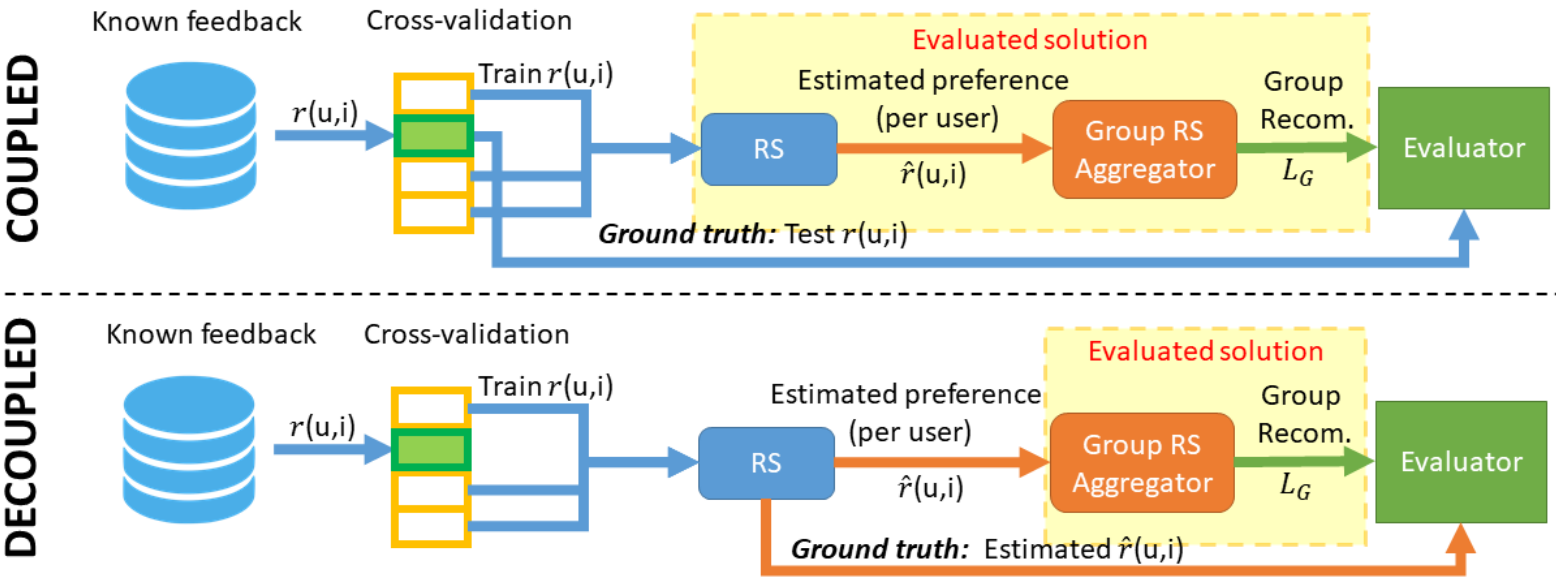
\includegraphics[width=5.5in]{img/coupled_decoupled_evaluation.png}
    \caption{Example of two main evaluation approaches from \cite{peska2021coupled}.}
    \label{fig:coupled_decoupled}
\end{figure}

% -------------------------------------------------------------------------------------
\subsection{Metrics}\label{subsec:07_experiments.evaluation.metrics}
% -------------------------------------------------------------------------------------

After running the group recommendation algorithm, we end up with a list of recommendations for each group. We now need to evaluate the performance of each algorithm.
For each group size, group type, and algorithm, we want to get a measure of how well they have performed.

Firstly, we need to get the ground truth from our underlying RS for each item and each group member.
Now for each group member and list of recommendations, we evaluate two metrics: normalized discounted cumulative gain (\textbf{nDCG}) and average relevance score (\textbf{AR}). We have chosen nDCG due to its popular use in our domain and a good representation of the probability of selection of an item based on the item's position in the list. AR metric has been chosen due to its simplicity and an overall good measure of performance for short lists of recommendations.

For each group and each user, we have \textbf{AR} and \textbf{nDCG} scores. Further, we calculate the aggregated per-group statistics for both of these metrics. We calculate \textbf{mean}, minimal user's score (\textbf{min}), and the ratio between minimal and maximal scores (\textbf{M/M}). All of these are valid fairness definitions on their own, depending on the definition of fairness as discussed in Chapter \ref{chap:fairness}. These metrics are also used in related literature \cite{GFAR-kaya2020}, \cite{sacharidis_2019_top_n_with_fairness}. Finally, we aggregate results for all groups together by calculating the mean of the metrics.

% -------------------------------------------------------------------------------------
\subsection{Evaluation use-cases}\label{subsec:07_experiments.evaluation.use_cases}
% -------------------------------------------------------------------------------------

In \cite{GFAR-kaya2020}, they focus only on the scenario of uniform groups, where each user is weighted uniformly. For our experiments, we are evaluating not only the \textbf{uniform} scenario but \textbf{weighted} and \textbf{long-term} scenarios as well.

In the \textbf{weighted scenario}, we randomly assign a weight to each of the group members (all summing up to a total of 1). This weight represents the non-uniform importance of each group member. This scenario is a relevant strategy for situations in structured groups where some members have a priority, such as a family with children watching a movie or a birthday party. This is an extension of the most respected person strategy described in \cite{most_respected_person}, with less rigid rules of only requiring weights to be in an interval of [0,1], with the total sum of weights in the group equal to 1.

In the \textbf{long-term scenario}, we assume that, in reality, the groups are more permanent with multiple instances of recommendation that are time separated. Such as a group of friends watching a movie every week or any other fixed group that consumes content together repeatedly. In this scenario, we want to prevent a systematic bias against one or multiple members and recommend items in the subsequent sessions with respect to the satisfaction and fairness of the previous sessions. We use the weights as in the previous weighted scenario and adjust them accordingly to satisfy the under-represented uses. We define the weights as a non-negative difference between the exactly proportional share of total relevance and the sum of relevance scores that the user has gained so far.

To evaluate the long-term scenario, we recommend items five times in a row, where after each row we calculate the appropriate weights and exclude the previously recommended items from further recommendation. After these five recommendation rows, we evaluate the mean utility for each user.


% -------------------------------------------------------------------------------------
\section{Evaluation setup} \label{sec:07_experiments.evaluation_setup}
% -------------------------------------------------------------------------------------
The experimental setup is an extended version from our \cite{our_ep_fuzz_da}. In the paper, we have used experiments from \cite{GFAR-kaya2020}, that we have extended with our algorithms and weighted and long-term recommendations.

Unfortunately, the original code from \cite{GFAR-kaya2020} we have worked with is quite proprietary and written in Java. For this work, we would have to extend it even further (compared to our work in \cite{our_ep_fuzz_da}) by adding the new group generation process that we have designed in Section \ref{sec:creation_of_artificial_groups}, new datasets, and a new matrix factorization. For convenience and further future research reusability, we have therefore made a decision to write all parts of the experiment in Python.

The main notable change from \cite{GFAR-kaya2020} is that we have modified the evaluation procedure. We use the decoupled evaluation instead of the coupled one as it gives an unfair advantage to algorithms that select the per-user best items and does not evaluate the underlying single-user RS in a coupled way as mentioned in Subsection \ref{subsec:07_experiments.evaluation.coupled_decoupled}.

Our experiments have 5 following steps.

% \begin{itemize}
    % \item \textbf{Data retrieval and processing:}
    \subsection{Data retrieval and processing}
        Unfortunately, as discussed in detail in Chapter \ref{chap:datasets}, we cannot host or append the used datasets directly to our code repository due to licensing. We have to therefore start with retrieving and processing the datasets.
        
        Run \path{./gather_datasets/downlad_and_transform.py} script directly if \newline you wish to retrieve the datasets manually. It supports Movie Lens, Netflix, KGrec, and Spotify datasets and performs cleanup and transformation to make further processing of the datasets as convenient as possible.

        The cleaning process transforms the datasets to a unified format with a single table of user ids, item ids, and ratings (if provided), normalizes and removes empty gaps from user and item ids, and validates the downloaded data.
    
        We have committed the weights that are outputted from the next step of matrix factorization to the repository. Therefore it is possible to skip this step if desired.

        
        
    % \item \textbf{Training matrix factorization algorithm:}
    \subsection{Training matrix factorization algorithm}
        We use two matrix factorization (MF) methods to generate our ground truths for the decoupled evaluation. First is our custom implementation of the highly parallel alternating least squares method (ALS) that we use for datasets with explicit ratings. The second is an implicit variation of the ALS method from a Python library Implicit \footnote{https://github.com/benfred/implicit} that we use for datasets with implicit ratings.

        As an output of this step, we get the two factors of MF, user and item factor matrix. We avoid saving the full target matrix due to the substantial size of the larger datasets, which would further increase our memory requirements. Instead, we calculate the ratings on the fly in the next steps.

        Run \path{./matrix_factorization/matrix_factorization.py} if you wish to calculate the matrix factorization manually.

        In our experiments, we use the following parameters for matrix factorization: number of iterations 15, random seed 42, regularization factor of 0.1, convergence threshold of 0.0001, and number of factors 50 for KGRec, 200 for Movie Lens, and 300 for Netflix and Spotify datasets. For KGRec and MovieLens datasets, we have selected the parameters similarly as in \cite{GFAR-kaya2020}. For other datasets, Netflix and Spotify, we have selected the parameters by hand based on a simple heuristic - the bigger and more complex the dataset, the higher the number of factors.
        
        Matrix factorization methods tend to degenerate when selecting the wrong parameters for the size of the factors, but the results for different types of groups (based on similarity PRS(M=1) and PRS(M=4)) do suggest that this is not the case, due to better results for groups with higher similarity (groups of more similar members are easier to satisfy). If the factors would degenerate and provide us only with flat ratings, then there would not be a difference in results for the two mentioned types of groups.

        We have committed the generated weights for all datasets into the code repository. Therefore it is possible to skip this step if desired. They are stored in a binary Numpy format with one exception for the Spotify dataset for which the item factor has reached the limit of GitHub LFS maximum file size. Therefore, we have zipped this dataset's factorization data in a standard .zip format.
        
    % \item \textbf{Creation of synthetic user groups:}
    \subsection{Creation of synthetic user groups}
        We have implemented 3 group creation strategies as already discussed in Section \ref{sec:creation_of_artificial_groups}. These are Random, Top-K, and Probability respecting similarity (PRS) algorithms. As shown in Figure \ref{fig:inter_group_means}, our method PRS nicely scales between the two extremes of Random and Top-K selection. We further assume that these two extremes do not often appear in real-world scenarios. Therefore, we have omitted them from our evaluation to simplify our experiments and only use groups created by the PRS algorithm.

        Run \path{./create_groups/create_random_groups.py} to create random groups \newline
        or run \path{./create_groups/create_topk_groups.py} to create Top-K groups \newline
        or run \path{./create_groups/create_prs_groups.py} if you wish to create PRS groups.
        
        We use PRS with two different settings of M, first at $M=1$ and second at $M=4$. Based on our analysis in \ref{subsec:04_creation_of_artificial_groups.evaluation}, we believe these two variants nicely represent the usual group setting.
        
        Further, for each setting, we generate 1000 groups in sizes 2, 3, 4, 6, and 8. We use 1000 candidates for each group, and lastly, we use 10,000 samples to get the dataset's similarity distribution.

        For weighted experiments, we additionally generate group weights as described in Subsection \ref{subsec:07_experiments.evaluation.use_cases}.
        
        Run \path{./create_groups/create_group_weights.py} if you wish to generate them manually.
    
    % \item \textbf{Running GRS algorithms:}
    \subsection{Running GRS algorithms}
        After the previous steps, we finally have all the required data to run GRS algorithm. We use the following algorithms from Chapter \ref{chap:related_work}: \textbf{AVG}, \textbf{LM}, \textbf{FAI}, \textbf{XPO\cite{sacharidis_2019_top_n_with_fairness}}, \textbf{NPO}, \textbf{GFAR\cite{GFAR-kaya2020}} together with \textbf{EP-FuzzDA} and is direct optimization variant \textbf{DHondtDO}.

        We use a computation optimization for all algorithms, where for each group member, we select their top 1000 candidate items (by rating), and then we compute the algorithm's item selection only on a joined set of these top items. Note that it is 1000 for each group member, so the number of candidate items in the set for the whole group will be bigger. For XPO and NPO, we use 30 candidate items instead of 1000 due to the computational complexity of those algorithms (this will be further discussed in \ref{sec:experiments.discussion}).

        Complete overview of all parameters for each algorithm:
        \begin{itemize}
            \item \textbf{AVG, LM, FAI}: candidate items = 1000
            \item \textbf{XPO, NPO}: candidate items = 30, monte Carlo trials = 100
            \item \textbf{GFAR}: candidate items = 1000, max relevant items = 100
            \item \textbf{EP-FuzzDA, DHondtDO}: candidate items = 1000, 
        \end{itemize}

        For each group and each algorithm, we get the top 10 items.

        Run \path{./experiments/run_algorithms.py},
        \newline
        \path{./experiments/run_weighted_algorithms.py} and
        \newline
        \path{./experiments/run_longterm_algorithms.py} to generate uniform, weighted and long-term experiments, respectively.
    
    % \item \textbf{Evaluation:}
    \subsection{Evaluation}
        The last step is an evaluation of the results. We have 4 datasets, 5 group sizes of 2, 3, 4, 6, 8. 2 types of groups, and 8 GRS algorithms. and 6 metrics combination as described in Subsection \ref{subsec:07_experiments.evaluation.metrics}.
        We evaluate these results in the following Jupyter notebooks under the directory \path{./evaluation/} directory. For uniform run \path{evaluation_uniform.ipynb}, 
 for weighted run \path{evaluation_weighted.ipynb} and for long-term \path{evaluation_longterm.ipynb}. These notebooks are meant to be run manually to get the results, but support an execution in the style of the previous scripts by running \path{jupyter}\kern 0.2em\path{run}\kern 0.2em\path{./evaluation/evaluation_uniform.ipunb}.
        
% \end{itemize}

% -------------------------------------------------------------------------------------
\section{Results}
% -------------------------------------------------------------------------------------

Due to the high number of datasets, we will present the efficacy on the Movie Lens (25M) dataset. Significant results of other datasets that differ from the Movie Lens dataset will be also discussed. Results for other datasets can be found in Appendix \ref{apendix:additional_results}.

% -------------------------------------------------------------------------------------
\subsection{Uniform scenario} \label{subsec:07_experiments.results.uniform}
% -------------------------------------------------------------------------------------

\begin{table}[!htbp]
    \centering
    \scalebox{0.76}{\hspace*{-1.2cm}{
    \begin{tabular}{ c | c c c | c c c || c c c | c c c}

\multicolumn{1}{c}{} & \multicolumn{6}{c}{PRS(M=1), group size s=2} & \multicolumn{6}{c}{PRS(M=4), group size s=2} \\
\multicolumn{1}{c}{} & \multicolumn{3}{c}{AR} & \multicolumn{3}{c}{nDCG} & \multicolumn{3}{c}{AR} & \multicolumn{3}{c}{nDCG} \\
& mean & min & M/M & mean & min & M/M & mean & min & M/M & mean & min & M/M \\
\hline
AVG & \textbf{64.75} & 49.19 & 0.67 & \underline{0.85} & \underline{0.78} & 0.85 & \textbf{66.11} & 50.50 & 0.69 & \underline{0.85} & \underline{0.78} & 0.86 \\
FAI & 56.05 & 48.45 & 0.79 & 0.76 & 0.71 & \underline{0.88} & 57.16 & 49.52 & 0.79 & 0.76 & 0.71 & \underline{0.88} \\
LM & 58.55 & \underline{55.68} & \underline{0.91} & 0.81 & 0.72 & 0.81 & 60.02 & \underline{57.21} & \underline{0.92} & 0.82 & 0.73 & 0.82 \\
XPO & 55.85 & 48.01 & 0.78 & 0.75 & 0.69 & 0.85 & 57.05 & 48.98 & 0.78 & 0.75 & 0.69 & 0.86 \\
NPO & 54.52 & 46.12 & 0.77 & 0.73 & 0.67 & 0.84 & 55.67 & 47.36 & 0.77 & 0.73 & 0.67 & 0.84 \\
GFAR & 48.55 & 43.38 & \textit{0.82} & 0.68 & 0.63 & \textit{0.86} & 49.43 & 44.14 & \textit{0.83} & 0.68 & 0.63 & \textit{0.87} \\
DHondtDO & \underline{64.06} & \textit{52.47} & 0.74 & \textbf{0.86} & \textbf{0.83} & \textbf{0.94} & \underline{65.43} & \textit{54.08} & 0.75 & \textbf{0.86} & \textbf{0.83} & \textbf{0.94} \\
EP-FuzzDA & \textit{59.61} & \textbf{57.00} & \textbf{0.92} & \textit{0.83} & \textit{0.76} & 0.83 & \textit{61.10} & \textbf{58.56} & \textbf{0.93} & \textit{0.83} & \textit{0.76} & 0.84 \\

\multicolumn{12}{c}{} \\
\multicolumn{1}{c}{} & \multicolumn{6}{c}{PRS(M=1), group size s=3} & \multicolumn{6}{c}{PRS(M=4), group size s=3} \\
\multicolumn{1}{c}{} & \multicolumn{3}{c}{AR} & \multicolumn{3}{c}{nDCG} & \multicolumn{3}{c}{AR} & \multicolumn{3}{c}{nDCG} \\
& mean & min & M/M & mean & min & M/M & mean & min & M/M & mean & min & M/M \\
\hline
AVG & \textbf{61.01} & 42.67 & 0.56 & \underline{0.78} & \underline{0.70} & \underline{0.81} & \textbf{61.30} & 44.04 & 0.58 & \underline{0.78} & \underline{0.71} & \underline{0.81} \\
FAI & 49.62 & 41.07 & 0.72 & 0.67 & 0.56 & 0.74 & 50.03 & 41.94 & 0.73 & 0.67 & 0.56 & 0.74 \\
LM & 53.67 & \underline{49.61} & \textbf{0.86} & 0.74 & 0.61 & 0.72 & 54.67 & \underline{50.80} & \textbf{0.87} & 0.74 & 0.63 & 0.73 \\
XPO & 49.88 & 40.81 & 0.71 & 0.67 & 0.56 & 0.73 & 50.35 & 41.73 & 0.72 & 0.67 & 0.57 & 0.74 \\
NPO & 47.95 & 38.68 & 0.69 & 0.64 & 0.53 & 0.70 & 48.49 & 39.33 & 0.70 & 0.65 & 0.53 & 0.71 \\
GFAR & 46.78 & 39.83 & \textit{0.75} & 0.65 & 0.55 & 0.74 & 47.27 & 40.56 & \textit{0.76} & 0.65 & 0.55 & 0.75 \\
DHondtDO & \underline{60.16} & \textit{46.00} & 0.64 & \textbf{0.79} & \textbf{0.75} & \textbf{0.90} & \underline{60.47} & \textit{47.25} & 0.66 & \textbf{0.79} & \textbf{0.74} & \textbf{0.90} \\
EP-FuzzDA & \textit{56.63} & \textbf{50.21} & \underline{0.82} & \textit{0.77} & \textit{0.67} & \textit{0.78} & \textit{57.29} & \textbf{51.76} & \underline{0.85} & \textit{0.77} & \textit{0.67} & \textit{0.79} \\

\multicolumn{12}{c}{} \\
\multicolumn{1}{c}{} & \multicolumn{6}{c}{PRS(M=1), group size s=4} & \multicolumn{6}{c}{PRS(M=4), group size s=4} \\
\multicolumn{1}{c}{} & \multicolumn{3}{c}{AR} & \multicolumn{3}{c}{nDCG} & \multicolumn{3}{c}{AR} & \multicolumn{3}{c}{nDCG} \\
& mean & min & M/M & mean & min & M/M & mean & min & M/M & mean & min & M/M \\
\hline
AVG & \textbf{57.48} & 39.52 & 0.51 & \underline{0.75} & \underline{0.66} & \underline{0.78} & \textbf{58.04} & 40.81 & 0.54 & \underline{0.74} & \underline{0.65} & \underline{0.78} \\
FAI & 45.73 & 36.95 & 0.67 & 0.62 & 0.49 & 0.65 & 46.21 & 37.44 & 0.68 & 0.62 & 0.48 & 0.65 \\
LM & 50.49 & \textbf{45.98} & \textbf{0.82} & 0.70 & 0.55 & 0.66 & 51.37 & \underline{47.03} & \textbf{0.83} & 0.70 & 0.56 & 0.68 \\
XPO & 46.57 & 37.09 & 0.66 & 0.63 & 0.49 & 0.65 & 46.97 & 37.48 & 0.67 & 0.63 & 0.49 & 0.66 \\
NPO & 44.52 & 34.98 & 0.64 & 0.61 & 0.46 & 0.61 & 44.69 & 35.09 & 0.65 & 0.60 & 0.45 & 0.62 \\
GFAR & 46.06 & 37.69 & \textit{0.69} & 0.64 & 0.50 & 0.65 & 46.34 & 38.11 & \textit{0.70} & 0.63 & 0.49 & 0.65 \\
DHondtDO & \underline{56.67} & \textit{42.49} & 0.59 & \textbf{0.75} & \textbf{0.70} & \textbf{0.86} & \underline{57.21} & \textit{43.78} & 0.62 & \textbf{0.74} & \textbf{0.68} & \textbf{0.85} \\
EP-FuzzDA & \textit{53.73} & \underline{45.89} & \underline{0.77} & \textit{0.74} & \textit{0.62} & \textit{0.73} & \textit{54.71} & \textbf{47.54} & \underline{0.79} & \textit{0.74} & \textit{0.62} & \textit{0.74} \\

\multicolumn{12}{c}{} \\
\multicolumn{1}{c}{} & \multicolumn{6}{c}{PRS(M=1), group size s=6} & \multicolumn{6}{c}{PRS(M=4), group size s=6} \\
\multicolumn{1}{c}{} & \multicolumn{3}{c}{AR} & \multicolumn{3}{c}{nDCG} & \multicolumn{3}{c}{AR} & \multicolumn{3}{c}{nDCG} \\
& mean & min & M/M & mean & min & M/M & mean & min & M/M & mean & min & M/M \\
\hline
AVG & \textbf{54.10} & 36.80 & 0.46 & \underline{0.70} & \underline{0.59} & \underline{0.73} & \textbf{54.69} & 37.94 & 0.49 & \underline{0.70} & \underline{0.59} & \underline{0.73} \\
FAI & 42.04 & 32.27 & 0.61 & 0.57 & 0.39 & 0.53 & 42.47 & 32.62 & 0.61 & 0.57 & 0.39 & 0.54 \\
LM & 47.47 & \textbf{42.51} & \textbf{0.78} & 0.66 & 0.48 & 0.59 & 48.16 & \underline{43.32} & \textbf{0.79} & 0.65 & 0.49 & 0.61 \\
XPO & 43.63 & 32.52 & 0.58 & 0.59 & 0.40 & 0.53 & 44.25 & 32.95 & 0.58 & 0.59 & 0.40 & 0.53 \\
NPO & 41.00 & 30.58 & 0.58 & 0.56 & 0.37 & 0.51 & 41.40 & 30.57 & 0.58 & 0.56 & 0.37 & 0.51 \\
GFAR & 44.16 & 33.86 & \textit{0.61} & 0.61 & 0.40 & 0.53 & 44.54 & 34.32 & \textit{0.62} & 0.60 & 0.41 & 0.54 \\
DHondtDO & \underline{53.27} & \textit{39.20} & 0.54 & \textbf{0.71} & \textbf{0.61} & \textbf{0.77} & \underline{53.87} & \textit{40.09} & 0.57 & \textbf{0.70} & \textbf{0.61} & \textbf{0.77} \\
EP-FuzzDA & \textit{51.03} & \underline{42.20} & \underline{0.70} & \textit{0.70} & \textit{0.54} & \textit{0.65} & \textit{51.84} & \textbf{43.32} & \underline{0.72} & \textit{0.70} & \textit{0.55} & \textit{0.67} \\

\multicolumn{12}{c}{} \\
\multicolumn{1}{c}{} & \multicolumn{6}{c}{PRS(M=1), group size s=8} & \multicolumn{6}{c}{PRS(M=4), group size s=8} \\
\multicolumn{1}{c}{} & \multicolumn{3}{c}{AR} & \multicolumn{3}{c}{nDCG} & \multicolumn{3}{c}{AR} & \multicolumn{3}{c}{nDCG} \\
& mean & min & M/M & mean & min & M/M & mean & min & M/M & mean & min & M/M \\
\hline
AVG & \textbf{51.76} & 35.51 & 0.45 & \textit{0.68} & \underline{0.54} & \underline{0.68} & \textbf{52.13} & 36.38 & 0.48 & \underline{0.68} & \underline{0.55} & \underline{0.68} \\
FAI & 39.89 & 29.15 & 0.56 & 0.55 & 0.32 & 0.45 & 40.11 & 29.52 & 0.57 & 0.55 & 0.34 & 0.46 \\
LM & 45.54 & \textbf{40.37} & \textbf{0.77} & 0.63 & 0.43 & 0.54 & 45.95 & \textbf{41.19} & \textbf{0.79} & 0.63 & 0.45 & 0.56 \\
XPO & 41.86 & 29.48 & 0.53 & 0.57 & 0.34 & 0.45 & 42.22 & 30.09 & 0.55 & 0.57 & 0.35 & 0.47 \\
NPO & 39.48 & 27.72 & 0.53 & 0.54 & 0.31 & 0.43 & 39.42 & 27.77 & 0.54 & 0.54 & 0.32 & 0.44 \\
GFAR & 42.17 & 31.37 & \textit{0.58} & 0.58 & 0.35 & 0.46 & 42.50 & 31.69 & \textit{0.59} & 0.58 & 0.37 & 0.49 \\
DHondtDO & \underline{51.10} & \textit{37.59} & 0.53 & \textbf{0.68} & \textbf{0.56} & \textbf{0.70} & \underline{51.49} & \textit{38.31} & 0.56 & \textbf{0.68} & \textbf{0.56} & \textbf{0.71} \\
EP-FuzzDA & \textit{49.34} & \underline{40.13} & \underline{0.67} & \underline{0.68} & \textit{0.49} & \textit{0.60} & \textit{49.91} & \underline{40.95} & \underline{0.69} & \textit{0.68} & \textit{0.51} & \textit{0.63} \\

\end{tabular}
    
    }}\hspace*{-1.3cm}
    \caption[Results of offline uniform evaluation on Movie Lens dataset]{Results of offline \textbf{uniform} evaluation on \textbf{MovieLens25M} dataset. The best results are in bold, the second-best are underscored, and the third-best results are in italic.}
    \label{table:7.results_uniform_ml}
\end{table}


In Table \ref{table:7.results_uniform_ml}, we can see that EP-FuzzDA performs well across all experimental metrics and group sizes. For AR metrics, the performance is mostly led by AVG and LM algorithms, where AVG dominates in AR mean, which is explainable due to its direct optimization of the highest average relevance. For AR min and M/M the performance is led by LM algorithm, with our EP-FuzzDA following with only a slight decrease in the performance and for smaller group sizes of 2 and 3 actually outperforming the LM algorithm. The slight edge of LM in these two metrics can be again explained by its direct optimization of the highest minimal relevance. Overall, we can say that our algorithm performs the best when evaluating the combination of mean, min, and M/M. It provides better mean average relevance values than LM and better min, M/M performance with only a slight decrease in mean AR compared to AVG.

For nDCG metrics, where the position of the items becomes important, it performs worse than the related DHondtDirect optimization, which performs more of a greedy recommendation strategy. Nevertheless, still, the performance is comparable to the best results.

For groups with more similarity (PRS, M=4) the results are comparable, with a slight improvement in performance for bigger but more similar groups. It is easier to recommend universally liked items when the preferences align more between the group members. For those situations, our algorithm's performance increases for AR min metric.

We conclude that, for the uniform evaluation scenario and the Movie Lens dataset, our EP-FuzzDA algorithm provides the highest fairness (in the context of our metrics) while maintaining the high relevance of the recommendation as measured by the mean AR and nDCG metrics.

Additionally, for the KGRec dataset (Table \ref{table:appendix.results_uniform_kgrec}), it provides recommendations with the best minimal and highest min/max score ratios for group sizes 4 and 6 and close to the best for the challenging group size 8. In more difficult scenarios of big and less similar groups $PRS(M=1)$ group size s=8, the algorithm performs well and is only dominated in those metrics by more specialized but naive algorithms (AVG, LM).

For the smaller MovieLens1M dataset (Table \ref{table:appendix.results_uniform_movie_lens_small}), and the Netflix dataset (Table \ref{table:appendix.results_uniform_netflix}), the results are analogical to the Movie Lens dataset.

And finally, for the Spotify dataset (Table \ref{table:appendix.results_uniform_spotify}), the results are slightly improved and are analogical to the KGRec dataset. This is interesting as it shows that for implicit datasets, the algorithm's performance seems to be better even for different sizes of the dataset (KGRec being the smallest and Spotify being the biggest).



% -------------------------------------------------------------------------------------
\subsection{Weighted scenario}
% -------------------------------------------------------------------------------------

\begin{table}[!ht]
    \centering
    \scalebox{0.82}{\hspace*{-1.2cm}{
    \begin{tabular}{ c | c c c | c c c || c c c | c c c}

\multicolumn{1}{c}{} & \multicolumn{6}{c}{PRS(M=1), group size s=3} & \multicolumn{6}{c}{PRS(M=4), group size s=3} \\
\multicolumn{1}{c}{} & \multicolumn{3}{c}{AR} & \multicolumn{3}{c}{nDCG} & \multicolumn{3}{c}{AR} & \multicolumn{3}{c}{nDCG} \\
& mean & corr & MAE & mean & corr & MAE & mean & corr & MAE & mean & corr & MAE \\
\hline
AVG-U & \textbf{61.01} & 0.01 & 0.17 & \textbf{0.78} & 0.01 & 0.15 & \textbf{61.30} & -0.02 & 0.17 & \textbf{0.78} & -0.02 & 0.15 \\
AVG & \underline{58.30} & 0.46 & 0.13 & 0.75 & 0.46 & \underline{0.11} & \underline{58.47} & 0.45 & 0.13 & 0.76 & 0.45 & \underline{0.11} \\
DHondtDO & 57.84 & \underline{0.46} & \underline{0.13} & \underline{0.76} & \underline{0.46} & 0.11 & 58.29 & \underline{0.45} & \underline{0.13} & \underline{0.76} & \underline{0.45} & 0.11 \\
EP-FuzzDA & 54.74 & \textbf{0.73} & \textbf{0.10} & 0.74 & \textbf{0.73} & \textbf{0.10} & 55.30 & \textbf{0.73} & \textbf{0.10} & 0.74 & \textbf{0.73} & \textbf{0.10} \\

\multicolumn{12}{c}{} \\
\multicolumn{1}{c}{} & \multicolumn{6}{c}{PRS(M=1), group size s=4} & \multicolumn{6}{c}{PRS(M=4), group size s=4} \\
\multicolumn{1}{c}{} & \multicolumn{3}{c}{AR} & \multicolumn{3}{c}{nDCG} & \multicolumn{3}{c}{AR} & \multicolumn{3}{c}{nDCG} \\
& mean & corr & MAE & mean & corr & MAE & mean & corr & MAE & mean & corr & MAE \\
\hline
AVG-U & \textbf{57.48} & 0.00 & 0.13 & \textbf{0.75} & 0.00 & 0.11 & \textbf{58.04} & -0.01 & 0.13 & \textbf{0.74} & -0.01 & 0.12 \\
AVG & \underline{55.13} & 0.43 & 0.11 & 0.72 & 0.43 & \underline{0.08} & \underline{55.39} & 0.46 & 0.10 & 0.71 & 0.46 & \underline{0.08} \\
DHondtDO & 54.79 & \underline{0.45} & \underline{0.10} & \underline{0.73} & \underline{0.45} & 0.09 & 54.89 & \underline{0.47} & \underline{0.10} & \underline{0.72} & \underline{0.47} & 0.09 \\
EP-FuzzDA & 52.45 & \textbf{0.65} & \textbf{0.08} & 0.72 & \textbf{0.65} & \textbf{0.08} & 53.16 & \textbf{0.65} & \textbf{0.08} & 0.71 & \textbf{0.65} & \textbf{0.08} \\

\multicolumn{12}{c}{} \\
\multicolumn{1}{c}{} & \multicolumn{6}{c}{PRS(M=1), group size s=6} & \multicolumn{6}{c}{PRS(M=4), group size s=6} \\
\multicolumn{1}{c}{} & \multicolumn{3}{c}{AR} & \multicolumn{3}{c}{nDCG} & \multicolumn{3}{c}{AR} & \multicolumn{3}{c}{nDCG} \\
& mean & corr & MAE & mean & corr & MAE & mean & corr & MAE & mean & corr & MAE \\
\hline
AVG-U & \textbf{54.10} & 0.02 & 0.09 & \textbf{0.70} & 0.02 & 0.08 & \textbf{54.69} & -0.02 & 0.09 & \textbf{0.70} & -0.02 & 0.08 \\
AVG & \underline{51.93} & 0.40 & 0.07 & 0.68 & 0.40 & \underline{0.06} & \underline{52.50} & 0.41 & 0.07 & 0.68 & 0.41 & \underline{0.06} \\
DHondtDO & 51.52 & \underline{0.42} & \underline{0.07} & \underline{0.68} & \underline{0.42} & 0.06 & 52.16 & \underline{0.43} & \underline{0.07} & \underline{0.68} & \underline{0.43} & 0.06 \\
EP-FuzzDA & 49.89 & \textbf{0.58} & \textbf{0.06} & 0.68 & \textbf{0.58} & \textbf{0.06} & 50.53 & \textbf{0.58} & \textbf{0.06} & 0.67 & \textbf{0.58} & \textbf{0.06} \\

\multicolumn{12}{c}{} \\
\multicolumn{1}{c}{} & \multicolumn{6}{c}{PRS(M=1), group size s=8} & \multicolumn{6}{c}{PRS(M=4), group size s=8} \\
\multicolumn{1}{c}{} & \multicolumn{3}{c}{AR} & \multicolumn{3}{c}{nDCG} & \multicolumn{3}{c}{AR} & \multicolumn{3}{c}{nDCG} \\
& mean & corr & MAE & mean & corr & MAE & mean & corr & MAE & mean & corr & MAE \\
\hline
AVG-U & \textbf{51.76} & 0.01 & 0.07 & \textbf{0.68} & 0.01 & 0.06 & \textbf{52.13} & 0.02 & 0.07 & \textbf{0.68} & 0.02 & 0.06 \\
AVG & \underline{49.83} & 0.40 & 0.06 & 0.65 & 0.40 & \textbf{0.05} & \underline{50.28} & 0.41 & 0.06 & 0.66 & 0.41 & \underline{0.05} \\
DHondtDO & 49.52 & \underline{0.42} & \underline{0.05} & \underline{0.66} & \underline{0.42} & 0.05 & 49.92 & \underline{0.43} & \underline{0.05} & \underline{0.66} & \underline{0.43} & 0.05 \\
EP-FuzzDA & 48.33 & \textbf{0.53} & \textbf{0.05} & 0.66 & \textbf{0.53} & \underline{0.05} & 48.82 & \textbf{0.55} & \textbf{0.05} & 0.66 & \textbf{0.55} & \textbf{0.05} \\

\end{tabular}
    
    }}\hspace*{-1.3cm}
    \caption[Results of offline weighted evaluation on Movie Lens dataset]{Results of offline \textbf{weighted} evaluation on \textbf{MovieLens25M} dataset. The best results are in bold. The second-best are underscored.}
    \label{table:7.results_weighted_ml}
\end{table}

In Table \ref{table:7.results_weighted_ml}, we see results for the weighted scenario. Our algorithm performs substantially better than AVG and DHondtDO for correlation and mean absolute error (MAE) metrics. These metrics tell us the correlation and MAE between the AR and nDCG for the group and the actual weight that has been randomly generated. We see that DHondtDO does a substantially worse job at weighing the group member preferences for a slight increase in the mean relevance performance compared to our algorithm. This is understandable. The act of weighing the relevance among the group members has to have some impact to the average performance. We have added the AVG-U algorithm, which is an AVG, but with the weights set to uniform as in the previous uniform scenario. We have added the AVG-U to serve as an upper bound for mean and a lower bound for correlation and MAE metrics. It has the best mean relevance performance but without the results correlating with the group weights.

Results for the KGRec dataset (Table \ref{table:appendix.results_weighted_kgrec}), 
the MovieLens1M dataset (Table \ref{table:appendix.results_weighted_movie_lens_small}), 
the Netflix dataset (Table \ref{table:appendix.results_weighted_netflix}), 
and the Spotify dataset (Table \ref{table:appendix.results_weighted_spotify})
are analogical to results for the MovieLens25M dataset.

% -------------------------------------------------------------------------------------
\subsection{Long-term scenario}
% -------------------------------------------------------------------------------------

\begin{table}[!ht]
    \centering
    \scalebox{0.82}{\hspace*{-1.2cm}{
    \begin{tabular}{ c | c c c | c c c || c c c | c c c }

\multicolumn{1}{c}{} & \multicolumn{6}{c}{PRS(M=1), group size s=3} & \multicolumn{6}{c}{PRS(M=4), group size s=3} \\
\multicolumn{1}{c}{} & \multicolumn{3}{c}{AR} & \multicolumn{3}{c}{nDCG} & \multicolumn{3}{c}{AR} & \multicolumn{3}{c}{nDCG} \\
& mean & min & M/M & mean & min & M/M & mean & min & M/M & mean & min & M/M \\
\hline
AVG-U & \underline{281.0} & 206.9 & 0.60 & \underline{2.09} & \underline{1.94} & \textbf{0.87} & \underline{282.4} & 213.0 & 0.62 & \underline{2.09} & \underline{1.95} & \textbf{0.87} \\
AVG & 264.6 & 233.3 & \underline{0.80} & 2.07 & 1.88 & \underline{0.84} & 268.7 & 239.0 & \underline{0.81} & 2.08 & 1.90 & \underline{0.85} \\
DHondtDO & \textbf{283.3} & \textbf{246.7} & 0.79 & \textbf{2.18} & \textbf{1.95} & 0.83 & \textbf{287.8} & \textbf{253.5} & 0.80 & \textbf{2.19} & \textbf{1.98} & 0.84 \\
EP-FuzzDA & 259.9 & \underline{241.2} & \textbf{0.89} & 2.05 & 1.71 & 0.73 & 263.4 & \underline{247.7} & \textbf{0.90} & 2.05 & 1.73 & 0.74 \\

\multicolumn{12}{c}{} \\
\multicolumn{1}{c}{} & \multicolumn{6}{c}{PRS(M=1), group size s=4} & \multicolumn{6}{c}{PRS(M=4), group size s=4} \\
\multicolumn{1}{c}{} & \multicolumn{3}{c}{AR} & \multicolumn{3}{c}{nDCG} & \multicolumn{3}{c}{AR} & \multicolumn{3}{c}{nDCG} \\
& mean & min & M/M & mean & min & M/M & mean & min & M/M & mean & min & M/M \\
\hline
AVG-U & \underline{266.7} & 194.0 & 0.55 & \underline{2.01} & \textbf{1.83} & \textbf{0.84} & \underline{268.7} & 200.2 & 0.58 & \underline{1.98} & \textbf{1.81} & \textbf{0.84} \\
AVG & 252.8 & 217.2 & \underline{0.76} & 2.00 & 1.74 & \underline{0.79} & 256.7 & 223.6 & \underline{0.78} & 1.98 & 1.74 & \underline{0.80} \\
DHondtDO & \textbf{267.7} & \textbf{227.9} & 0.76 & \textbf{2.09} & \underline{1.79} & 0.77 & \textbf{273.2} & \textbf{235.4} & 0.77 & \textbf{2.07} & \underline{1.80} & 0.78 \\
EP-FuzzDA & 249.6 & \underline{222.9} & \textbf{0.82} & 1.99 & 1.59 & 0.69 & 253.3 & \underline{229.9} & \textbf{0.85} & 1.96 & 1.60 & 0.70 \\

\multicolumn{12}{c}{} \\
\multicolumn{1}{c}{} & \multicolumn{6}{c}{PRS(M=1), group size s=6} & \multicolumn{6}{c}{PRS(M=4), group size s=6} \\
\multicolumn{1}{c}{} & \multicolumn{3}{c}{AR} & \multicolumn{3}{c}{nDCG} & \multicolumn{3}{c}{AR} & \multicolumn{3}{c}{nDCG} \\
& mean & min & M/M & mean & min & M/M & mean & min & M/M & mean & min & M/M \\
\hline
AVG-U & \underline{252.9} & 182.6 & 0.51 & 1.89 & \textbf{1.66} & \textbf{0.78} & \underline{255.2} & 187.5 & 0.54 & \underline{1.88} & \textbf{1.65} & \textbf{0.78} \\
AVG & 241.1 & 203.3 & \underline{0.73} & \underline{1.89} & 1.52 & \underline{0.69} & 244.7 & 207.9 & \underline{0.74} & 1.88 & 1.54 & \underline{0.71} \\
DHondtDO & \textbf{253.7} & \textbf{211.7} & 0.72 & \textbf{1.97} & \underline{1.55} & 0.68 & \textbf{258.2} & \textbf{217.2} & 0.74 & \textbf{1.96} & \underline{1.57} & 0.69 \\
EP-FuzzDA & 239.0 & \underline{206.2} & \textbf{0.76} & 1.88 & 1.40 & 0.62 & 242.3 & \underline{211.7} & \textbf{0.78} & 1.87 & 1.43 & 0.64 \\

\multicolumn{12}{c}{} \\
\multicolumn{1}{c}{} & \multicolumn{6}{c}{PRS(M=1), group size s=8} & \multicolumn{6}{c}{PRS(M=4), group size s=8} \\
\multicolumn{1}{c}{} & \multicolumn{3}{c}{AR} & \multicolumn{3}{c}{nDCG} & \multicolumn{3}{c}{AR} & \multicolumn{3}{c}{nDCG} \\
& mean & min & M/M & mean & min & M/M & mean & min & M/M & mean & min & M/M \\
\hline
AVG-U & \underline{243.5} & 176.9 & 0.50 & 1.83 & \textbf{1.53} & \textbf{0.72} & \underline{244.7} & 181.1 & 0.53 & 1.84 & \textbf{1.54} & \textbf{0.73} \\
AVG & 234.5 & 195.2 & \underline{0.71} & \underline{1.84} & 1.40 & \underline{0.64} & 236.7 & 199.2 & \underline{0.73} & \underline{1.84} & 1.44 & \underline{0.66} \\
DHondtDO & \textbf{245.5} & \textbf{202.6} & 0.71 & \textbf{1.90} & \underline{1.42} & 0.62 & \textbf{248.3} & \textbf{206.3} & 0.72 & \textbf{1.91} & \underline{1.46} & 0.64 \\
EP-FuzzDA & 232.4 & \underline{197.4} & \textbf{0.73} & 1.83 & 1.30 & 0.57 & 234.5 & \underline{201.2} & \textbf{0.75} & 1.83 & 1.35 & 0.60 \\

\end{tabular}
    
    }}\hspace*{-1.3cm}
    \caption[Results of offline long-term evaluation on Netflix dataset]{Results of offline \textbf{long-term} evaluation on \textbf{MovieLens25M} dataset. The best results are in bold, second-best are underscored.}
    \label{table:7.results_longterm_ml}
\end{table}

Interestingly, the results for the long-term scenario are different from the weighted scenario. We would expect that if an algorithm can better correlate the provided relevance with the provided weights, then it will perform better across the board in the long-term scenario. But, as we can see in Table \ref{table:7.results_longterm_ml}, DHondtDO dominates in mean and min AR metrics. EP-FuzzDA dominates in M/M AR metric. It balances the preference better than other algorithms, as discussed in the weighted scenario. This leads to better M/M AR performance because it provides fairer recommendations but for the price of decreased mean performance. We have checked the weights calculated after each round, and for EP-FuzzDA, they stay the most uniform, which tells us that the algorithm is doing a good job of maintaining fairness across the group members.

The results look analogical for the additional datasets, the KGRec dataset (Table \ref{table:appendix.results_longterm_kgrec}), 
the MovieLens1M dataset (Table \ref{table:appendix.results_longterm_movie_lens_small}), 
and the Spotify dataset (Table \ref{table:appendix.results_longterm_spotify}) 
except for the Netflix dataset (Table \ref{table:appendix.results_longterm_netflix}), where for groups with sizes over 6, the fairness performance of the M/M AR metric drops slightly.

% -------------------------------------------------------------------------------------
\section{Discussion} \label{sec:experiments.discussion}
% -------------------------------------------------------------------------------------

The GFAR algorithm performs poorly in our tests compared to the original research in \cite{GFAR-kaya2020}. This is probably caused by the different evaluation types as mentioned in Subsection \ref{subsec:07_experiments.evaluation.coupled_decoupled}, we use the decoupled evaluation, contrary to the original paper where they used the coupled evaluation. As discussed in our research in \cite{peska2021coupled}, it is possible that due to GFAR's use of Borda count as the relevance selection criteria, there could have been a popularity bias at play. The coupled evaluation requires that we have data in the testing part of our dataset for our recommended items. We are likelier to have a rating for popular items due to the popularity bias. GFAR commonly selects items that are best or among the best items for a user. Therefore the probability that we have data in the testing data (for coupled) is higher. This can lead to an unfair advantage in the coupled evaluation compared to other algorithms. On the other hand, in decoupled evaluation, we have estimated ratings for all pairs of users and items. Therefore, we can equally evaluate the selected items for all algorithms without this popularity bias affecting our results.

Another explanation for why GFAR is not performing well in our experiments can be the parameter selection. The algorithm calculates the probability of user satisfaction after each recommended item, which is then used to adjust the relevance probability of the candidate items in the next step. But for a higher number of maximal relevance items (how many items from the top-p of each candidate will be awarded the Borda rating), these probabilities are small and therefore push very little to balance the inter-group relevance inequalities from the previously recommended items. If one person in a big group differs in their preference from the rest, then GFAR won't push hard enough to satisfy this person at some point, especially if other members are in preference consensus.

XPO and NPO algorithms are not performing well in our setup. Similar to the already discussed GFAR algorithm. For all experiments, we use a randomly selected subset of 1000 candidate items (for each user, then joining these candidate lists together) from which we select the top 10. This is an optimization for performance reasons. Unfortunately, XPO and NPO do not scale well in settings where many candidate items are presented to the algorithm. This is due to internally considering all tuples of the candidate items and comparing them using random trials (details can be found in Subsection \ref{subsec:03_advanced_methods.xpo}). We had to therefore limit the candidate items to 30 (instead of 1000), and even that caused the XPO (and NPO) to remain the computationally slowest algorithms. An increase from 30 to only 100 candidate items resulted in 10 times worse computational performance, and we have therefore limited XPO and NPO algorithms to only 30 candidate items. Naturally, this leads to a lesser rating performance due to a lower selection pool.

The performance of our algorithm in the long-term evaluation was a little surprising. On the one hand, it can handle weighing well, as seen in the weighted scenario, but on the other hand, the average rating performance does not translate well to the long-term scenario. This is probably due to the algorithm pushing too hard to achieve the highest amount of fairness, even for a decrease in AR and nDCG mean and min performance. One possible way to suppress this could be to decrease the effect of the weights. However, then, again, the definition of fairness must be considered. If we require the most balanced performance, then our algorithm performs the best (with regard to the AR M/M metric).

Additionally, the performance of our algorithm in the long-term evaluation could be explained by the way how the experiment was set up. We calculate the weights for the next run from the previously recommended items. Based on the ratio of average ratings between the group members, we set the weights for the next iteration. But we also exclude the already recommended items from the next run. These already recommended items are better than the rest of our candidates (why they have been selected). Therefore we, in a way, overestimate the potential future ratings that we can receive. Therefore it is possible that in the current setup of this scenario, the algorithms that do not conform to the desired weights that much will get an edge over our algorithm, which, as shown by the results of the weighted scenario, does balance the preference based on weights the most.

We have observed slightly better performance in the uniform scenario for the two implicit datasets (KGRec and Spotify) compared to the explicit datasets (Movie Lens and Netflix). This could be due to overall better performance on this type of data, or it could also be a difference in our underlying matrix factorization algorithm.

Lastly, the performance seems to be quite analogical (with small deviations) over the different datasets, which widely differ in size. The same cannot be said about XPO and NPO algorithms, which in our current setting (as mentioned above) perform considerably worse when we compare the performance on the KGRec dataset (smallest) and the Spotify dataset (largest).


% -------------------------------------------------------------------------------------
\section{Reproducibility}
% -------------------------------------------------------------------------------------

Throughout our research, we encountered multiple situations when the experiments from the literature were hard to replicate and reuse. We have therefore taken increased care to provide an easy and convenient way to run all the experiments found in this work.

Firstly, we have selected Python as our programming language due to being the most popular and most used language in the data science domain.
Secondly, we have versioned all experiments in a single GitHub repository at \newline\href{https://github.com/LadislavMalecek/MasterThesisAnalysis}{github.com/LadislavMalecek/MasterThesisAnalysis}. And Lastly, we have created a convenient reproducibility shell script \path{run_experiments.sh} which can be found in the Git repository, mentioned at the beginning of this chapter.

Requirements:
\begin{itemize}
    \item Python 3.9
    \item Poetry - Python package manager
    \item 60 GB of disk space - storing the datasets and intermediate results
    \item 16 GB of ram (less if only running the smaller datasets (KGrec, Movielens-small)
    \item internet connection
\end{itemize}

After installing Python and poetry, clone the repository and run the provided shell script. Some of our more compute-heavy calculations, such as the matrix factorization, can utilize multi-core processing. Therefore, using a multi-core machine is advised (but not necessary).

% We provide a detailed structure of the repository:
Documentation of the repository structure can be found also in \path{./readme.md}. Each script is self-documenting, use the parameter \path{--help} to get more information about all usable parameters and default values.

The git repository has the following structure (only mentioning the most important files, which are mentioned in Section \ref{sec:07_experiments.evaluation_setup}:

\begin{forest}
  for tree={
    font=\ttfamily,
    grow'=0,
    child anchor=west,
    parent anchor=south,
    anchor=west,
    calign=first,
    edge path={
      \noexpand\path [draw, \forestoption{edge}]
      (!u.south west) +(7.5pt,0) |- node[fill,inner sep=1.25pt] {} (.child anchor)\forestoption{edge label};
    },
    before typesetting nodes={
      if n=1
        {insert before={[,phantom]}}
        {}
    },
    fit=band,
    before computing xy={l=15pt},
  }
[
  [create\_groups
    [create\_prs\_groups.py]
    [create\_random\_groups.py]
    [create\_topk\_groups.py]
  ]
  [datasets
    [kgrec]
    [movie\_lens]
    [movie\_lens\_small]
    [netflix]
    [spotify]
  ]
  [gather\_datasets
    [download\_and\_transform.py]
  ]
  [evaluation
    [evaluation\_longterm.ipynb]
    [evaluation\_uniform.ipynb]
    [evaluation\_weighted.ipynb]
  ]
  [experiments
    [run\_longterm\_algorithms.py]
    [run\_uniform\_algorithms.py]
    [run\_weighted\_algorithms.py]
  ]
  [matrix\_factorization
    [matrix\_factorization.py]
  ]
  [run\_experiments.sh]
]
\end{forest}